% Danish redrawing of the annotated box plot (same labels as figure/boxplot.png).
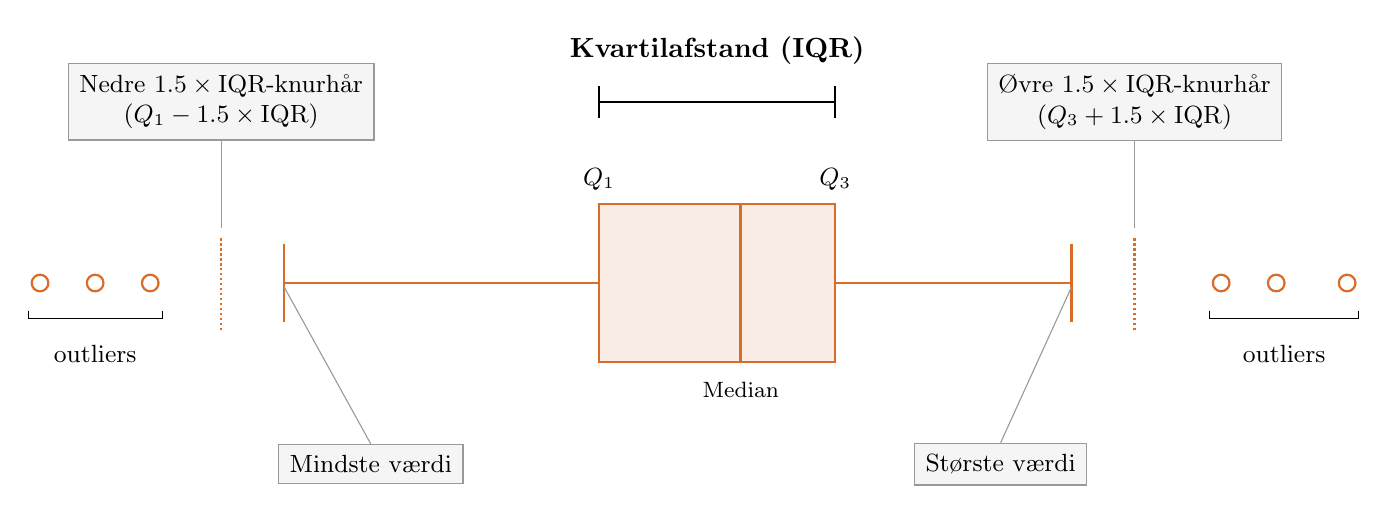
\begin{tikzpicture}[x=1cm, y=1cm, font=\small,
    lbl/.style={draw=black!40, fill=black!4, align=center, inner sep=4pt}]
  \definecolor{bxorange}{RGB}{217,108,40}
  % fences (1.5 x IQR) and whiskers
  \draw[bxorange, thick, densely dotted] (-3.3,-0.6) -- (-3.3,0.6);
  \draw[bxorange, thick, densely dotted] (8.3,-0.6) -- (8.3,0.6);
  \draw[bxorange, thick] (-2.5,0) -- (1.5,0) (4.5,0) -- (7.5,0);
  \draw[bxorange, thick] (-2.5,-0.5) -- (-2.5,0.5) (7.5,-0.5) -- (7.5,0.5);
  % box and median
  \draw[bxorange, thick, fill=bxorange!12] (1.5,-1) rectangle (4.5,1);
  \draw[bxorange, very thick] (3.3,-1) -- (3.3,1);
  \node[font=\footnotesize] at (3.3,-1.35) {Median};
  \node[anchor=south] at (1.5,1.05) {$Q_1$};
  \node[anchor=south] at (4.5,1.05) {$Q_3$};
  % IQR bracket
  \draw[thick] (1.5,2.3) -- (4.5,2.3) (1.5,2.1) -- (1.5,2.5) (4.5,2.1) -- (4.5,2.5);
  \node[font=\bfseries] at (3,2.95) {Kvartilafstand (IQR)};
  % outliers
  \foreach \x in {-5.6,-4.9,-4.2} \draw[bxorange, thick] (\x,0) circle (3pt);
  \foreach \x in {9.4,10.1,11.0} \draw[bxorange, thick] (\x,0) circle (3pt);
  \draw (-5.75,-0.35) to[out=-90,in=90] (-5.75,-0.45) -- (-4.05,-0.45) to[out=90,in=-90] (-4.05,-0.35);
  \draw (9.25,-0.35) to[out=-90,in=90] (9.25,-0.45) -- (11.15,-0.45) to[out=90,in=-90] (11.15,-0.35);
  \node at (-4.9,-0.9) {outliers};
  \node at (10.2,-0.9) {outliers};
  % labelled boxes
  \node[lbl] (lo) at (-3.3,2.3) {Nedre $1.5\times\mathrm{IQR}$-knurhår\\$(Q_1 - 1.5 \times \mathrm{IQR})$};
  \node[lbl] (hi) at (8.3,2.3) {Øvre $1.5\times\mathrm{IQR}$-knurhår\\$(Q_3 + 1.5 \times \mathrm{IQR})$};
  \draw[black!40] (lo.south) -- (-3.3,0.7) (hi.south) -- (8.3,0.7);
  \node[lbl] (mn) at (-1.4,-2.3) {Mindste værdi};
  \node[lbl] (mx) at (6.6,-2.3) {Største værdi};
  \draw[black!40] (mn.north) -- (-2.5,-0.05) (mx.north) -- (7.5,-0.05);
\end{tikzpicture}
